\documentclass[journal,twoside,web]{ieeecolor}

\usepackage{generic}
\usepackage{cite}
\usepackage{amsmath,amssymb,amsfonts}
\usepackage{graphicx}
\usepackage{xcolor}
\usepackage{booktabs}
\usepackage{multirow}
\usepackage{makecell}
\usepackage{array}
\usepackage{tabularx}
\usepackage{threeparttable}
\usepackage[caption=false,font=footnotesize]{subfig}
\usepackage{tikz}
\usetikzlibrary{arrows.meta,positioning,calc}
\usepackage{stfloats}
\usepackage{url}
\usepackage{hyperref}
\hypersetup{
  hidelinks,
  pdftitle={Commit or Abstain: Consensus Routing of Skip Evidence for Medical Image Segmentation},
  pdfauthor={Anonymous},
  pdfkeywords={abstention, evidence routing, medical image segmentation, normalized convolution, skip connections}
}

\graphicspath{{figures/}}
\setlength{\emergencystretch}{2em}
\renewcommand{\arraystretch}{1.08}

% Every result of the redesigned model is a placeholder until the Phase-3 runs finish (SPEC_v1 §8).
\newcommand{\TODO}[1]{\textcolor{red}{[TODO: #1]}}
\newcommand{\STALE}[1]{\textcolor{red}{#1}}

\def\BibTeX{{\rm B\kern-.05em{\sc i\kern-.025em b}\kern-.08em
    T\kern-.1667em\lower.7ex\hbox{E}\kern-.125emX}}

\markboth{IEEE Journal of Biomedical and Health Informatics}%
{Anonymous Author(s): Commit or Abstain: Consensus Routing of Skip Evidence for Medical Image Segmentation}

\begin{document}
\setlength{\floatsep}{8pt plus 2pt minus 2pt}
\setlength{\textfloatsep}{10pt plus 2pt minus 4pt}
\setlength{\abovecaptionskip}{6pt}

\title{Commit or Abstain: Consensus Routing of Skip Evidence for Medical Image Segmentation}

\author{Anonymous Author(s)
\thanks{Author names, affiliations, and funding information are omitted for double-blind review.}
\thanks{The design evaluated in this article is denoted ACRE-C (commit-or-abstain consensus routing of evidence); the code name of the model class is UKAN\_V2.}}

\maketitle

\begin{abstract}
Encoder--decoder segmenters recover a high-resolution mask by adding, at every decoder scale, an upsampled decoder feature to the encoder feature of the same resolution. This addition transports target evidence, its surroundings, and undecided evidence with the same weight, leaving the decoder to separate them at the boundary. Earlier selective designs aggregate neighbours without normalising by the weight that reached a location, and give the undecided state no operational role. We treat skip fusion as a vote. A controller formed once on the deepest convolutional feature assigns each cell a polarity and an abstention; the abstention has no target and is shaped only by its usefulness for routing. At every decoder scale, commitment-weighted normalised convolution forms a foreground and a background consensus over committed neighbours, locally and image-wide, and the abstention routes the evidence to one of two small experts. Every component is the identity at initialisation; the skip is never gated. It adds $0.39$ million parameters, $16\%$ more multiply--accumulate operations and $43\%$ more inference latency, to a compact Kolmogorov--Arnold encoder--decoder. We evaluate it on ultrasound, gland histology, and two colonoscopy collections under identical splits, budgets, and seeds. Against the re-trained backbone, three-seed mean test intersection over union changes by $+0.36$ on glands; \STALE{on the polyp collections and ultrasound the previous-protocol means are $+0.62$, $+2.10$ and $-0.45$ and will be replaced.} \STALE{Ablations (previous protocol): removing the no-decision state costs 0.7 points while fixing it to the full margin costs none.} A soft third routing state, not a learned one, is what makes the routing useful.
\end{abstract}

\begin{IEEEkeywords}
Abstention, evidence routing, medical image segmentation, normalised convolution, skip connections.
\end{IEEEkeywords}

\noindent\textcolor{red}{Transition draft (2026-09-05). The evaluation has been moved to an $80/10/10$ protocol with a test partition never used for training or model selection. GlaS results below are test-partition values. Red-marked numbers are values from the previous $80/20$ protocol that will be replaced as the corresponding re-training runs finish.}

\section{Introduction}
\label{sec:introduction}

\IEEEPARstart{U}{-shaped} segmenters recover a high-resolution mask by fusing, at every decoder scale, an upsampled decoder feature with the encoder feature of the same resolution~\cite{ronneberger2015unet,zhou2020unetpp}. Whether the backbone is convolutional, transformer-based~\cite{chen2021transunet,cao2023swinunet}, state-space~\cite{ruan2024umamba}, or built from Kolmogorov--Arnold network (KAN) blocks~\cite{li2025ukan}, this fusion is almost always an addition or a concatenation. The operation is agnostic to what the skip feature means: a response that supports the target, a response that supports its surroundings, and a response whose role is genuinely undecided are transported with the same weight. In breast ultrasound, colon histology, and colonoscopy---the settings studied here---the undecided class is large. Speckle and acoustic shadow blur lesion margins, packed glands share texture with their lumina, and specular glare and low mucosal contrast alter the appearance of polyps. Homogeneous transport carries all three kinds of evidence into the decoder and leaves the decoder to sort them out at the one place where an error is hardest to undo: the boundary.

A line of recent work makes the transport selective by conditioning it on a deep semantic state. ConDSeg decouples a deep feature into foreground, background, and uncertainty branches and lets the first two generate per-pixel involution-style kernels for the skip features~\cite{lei2025condseg}; contrast- and cluster-based context operators relate spatially separated responses to sharpen low-contrast regions~\cite{zhu2025ccvim}; boundary-band and distance-based objectives increase sensitivity to contour displacement~\cite{kervadec2019boundary,karimi2019reducing,wang2022banet}; attention gates and channel-wise skip re-weighting suppress irrelevant encoder responses~\cite{oktay2018attention,wang2022uctransnet,luo2025tamosc}. We regard this evidence-routing line as the right question and build on it, but three problems remain open in its current designs. First, the aggregation is \emph{unnormalised}: predicted per-pixel kernels are applied by unfold--fold without dividing by the total weight that reached a location, so the magnitude of the fused feature depends on how many neighbours voted, not only on what they voted for, and the skip signal itself is rescaled by a learned gate. Second, the third semantic state has \emph{no explicit operational meaning}: it is either fed to the decoder as one more channel or regularised through a foreground--background product penalty, so nothing in the architecture treats ``no decision'' differently from a weak decision. Third, the auxiliary losses \emph{compete} with the task: an ambiguity branch supervised by a loss acquires a loss-optimal value that need not be the value most useful for routing, and a boundary term whose normalisation follows the band area can dominate the objective on images with thin targets. In a preliminary instantiation of this recipe on the same backbone we observed dataset-dependent behaviour, including a mean decrease on CVC-ClinicDB; we hypothesise, without claiming a causal proof, that these three properties contributed.

This article proposes to treat skip fusion as a \emph{vote}. A lightweight controller, formed once on the deepest convolutional feature, gives every $8\times8$ cell a polarity $q\in(0,1)$---does the cell belong to the object?---and an abstention $m_a$, the fraction of the cell's commitment margin $\mu = 1-|2q-1|$ that it declines to commit. Polarity is supervised by soft cell occupancy; abstention has no target at all, because the controller loss is flat in the abstention by construction, so whatever abstention pattern emerges is shaped only by its usefulness downstream. At every decoder scale the baseline evidence $u = \mathrm{up} + \mathrm{skip}$ is kept intact, and two polarity-partitioned consensus fields $m^{+}$ and $m^{-}$ are formed by commitment-weighted normalised convolution: each is a convex combination of $u$ over neighbours that committed to foreground or to background, respectively, and abstaining pixels do not vote. The same operator taken image-wide yields $G^{+}$ and $G^{-}$, what committed foreground and background look like in this image. The abstention then routes the evidence between two small experts: a committed pixel receives a learned pull toward the consensus of its own polarity ($f_c$), an abstaining pixel receives the contrast between both consensuses ($f_a$), and the following KAN or convolutional block makes the decision. Every component is identity at initialisation, convex where it averages, and bounded where it gains. The skip is never multiplied by a gate; its detail band can at most be halved; and the learned residual is bounded by the expert norms, which we log, and by the abstention mass. We call the design ACRE-C, Commit-or-Abstain Consensus Routing of Evidence, and instantiate it on U-KAN as U-KAN\,+\,ACRE-C.

We acknowledge that ACRE-C is assembled from known primitives: normalised convolution with a certainty map, a two-expert mixture, an abstention output, a fixed low-/high-pass split of the skip, and a boundary-band-weighted cross-entropy. Section~\ref{sec:related} states for each what is shared and what differs; the contribution lies in how the primitives are coupled, and in the constraints that make the coupling safe. Specifically:
\begin{itemize}
    \item \textbf{A commit-or-abstain formulation of skip fusion.} A single controller yields commitment masses $(m_{fg}, m_{bg}, m_a)$ on the simplex through a $(q,\rho)$ parameterisation whose readout $m_{fg}+\tfrac{1}{2}m_a\equiv q$ holds by identity. The controller loss $\mathcal{L}_{\mathrm{ctrl}}$ acts on the polarity logit only, so its gradient with respect to the abstention is exactly zero and abstention is a routing variable and nothing else.
    \item \textbf{A consensus router with a bounded departure from the baseline.} Polarity-partitioned normalised-convolution consensus fields, local and image-wide at all four scales, are consumed by two zero-initialised experts routed by the abstention mass. The router adds 0.39\,M parameters to U-KAN (6.748\,M in total) and approximately 0.85\,GFLOPs at $256\times256$ input% calflops on the training server (2026-09-03, test_unit_v2.py [i]): 5.328 -> 6.177 GFLOPs, i.e. +0.85 G (+16%)
    , and reduces to $\mathrm{up}+\mathrm{skip}$ when all switches are off.
    \item \textbf{An objective that does not compete with the task.} A cell-occupancy commit loss anchors the polarity, and a focus loss re-weights the segmentation cross-entropy on the union of the ground-truth boundary band and the controller's own (detached) abstention, with a band normalisation floored at $\rho_f$ so that no pixel is up-weighted by more than a fixed factor. No morphology, distance transform, or schedule is used.
    \item \textbf{A controlled evaluation.} We compare U-KAN\,+\,ACRE-C against the re-trained U-KAN on BUSI, GlaS, CVC-ClinicDB, and Kvasir-SEG under identical 80/20 splits, training budgets, and three data seeds, with a cumulative ablation and side ablations that test whether a learned third state is necessary and whether the routing actually uses it. Eleven of the twelve seed-level comparisons of best validation IoU favour ACRE-C (three-seed means $+0.70$ GlaS, $+0.62$ CVC-ClinicDB, $+2.10$ Kvasir-SEG, $-0.45$ BUSI); removing the abstention costs $0.68$ points and fixing it to a full margin costs $0.23$ on GlaS, and the spatial standard deviation of $\rho$ stays between $0.05$ and $0.13$ on every screening run.
\end{itemize}
All reported numbers are validation results under the backbone's public protocol, and we make no claim of state-of-the-art performance; the aim is to establish whether normalised, abstention-routed skip fusion recovers the baseline where earlier evidence routing regressed and improves on it where it did not.

\section{Related Work}
\label{sec:related}

\subsection{Compact Backbones for Medical Image Segmentation}

U-Net and its nested and attention-gated variants established the encoder--decoder pattern in which semantic abstraction is recovered to full resolution through skip connections~\cite{ronneberger2015unet,zhou2020unetpp,oktay2018attention}. Later backbones enlarged the receptive field with self-attention~\cite{chen2021transunet,cao2023swinunet} or state-space operators~\cite{ruan2024umamba}, nnU-Net made the configured pipeline itself a determinant of accuracy~\cite{isensee2021nnunet}, and U-KAN replaces selected multilayer perceptrons in the deep tokenised stages by learnable spline transformations~\cite{li2025ukan}. All alter the representation operator; the fusion of encoder and decoder evidence remains an addition or a concatenation. We keep U-KAN unchanged and change only its four fusion points, so that any difference is attributable to how evidence is transported rather than to how it is represented.

\subsection{Selective Skip Fusion and Evidence Routing}

Several designs make the skip pathway selective. Attention gates re-weight encoder responses by a decoder-conditioned scalar map~\cite{oktay2018attention}; UCTransNet aligns encoder and decoder channels by cross-scale channel attention~\cite{wang2022uctransnet}; TA-MoSC treats skip selection as sparse expert routing driven by decoder preference~\cite{luo2025tamosc}; frequency-aware fusion predicts spatially varying low-pass filters for the decoder path and high-pass filters for the encoder path~\cite{chen2025freqfusion}; spatially adaptive normalisation and feature-wise linear modulation condition a feature by a learned scale and shift, per pixel from a semantic map~\cite{park2019spade} or per channel from a global vector~\cite{perez2018film}. In all of them the skip is scaled or filtered as a whole; ACRE-C scales only its detail band, within $(\tfrac12,\tfrac32)$, and otherwise lets the deep state decide only who votes and who reads.

The closest line decouples a deep feature into semantic states and lets those states steer the fusion. ConDSeg predicts foreground, background, and uncertainty branches, uses the first two to generate per-pixel aggregation kernels in the spirit of involution~\cite{li2021involution} that are applied to the skip by an unfold--fold aggregation, and regularises the branches with a penalty on the overlap of the foreground and background maps~\cite{lei2025condseg}. Context clustering combined with a state-space backbone relates distant responses through cluster centres to sharpen low-contrast regions~\cite{zhu2025ccvim}, and boundary-oriented objectives increase sensitivity to contour displacement~\cite{kervadec2019boundary,karimi2019reducing,wang2022banet}. ACRE-C belongs to this evidence-routing line and differs from ConDSeg in three places that Section~\ref{sec:method} makes precise: per-pixel generated kernels and unnormalised fold aggregation are replaced by a shared kernel with commitment-normalised averaging; the third state has an operational role, in that it does not vote and decides which expert reads the evidence, instead of being a regulariser; and the auxiliary objective acts on the polarity logit and on a re-weighted task loss only, so that no branch acquires a loss-optimal value that competes with its routing role.

\subsection{Normalised Convolution, Abstention, and Mixtures of Experts}

Normalised convolution filters a signal together with a certainty map and divides the filtered signal by the filtered certainty, so that uncertain samples contribute proportionally less and the output remains a convex combination of the inputs~\cite{knutsson1993normalized}. Used here with one learned certainty map per polarity, each output is a consensus of the neighbours that committed to the same class. The reject option~\cite{chow1970reject} and selective prediction~\cite{geifman2017selective} let a classifier decline to decide and supervise that decision against an error--coverage trade-off; our abstention is an internal routing variable that is never evaluated as a decision, has no target and no coverage constraint, and is shaped by the segmentation loss alone. Mixtures of experts weight several sub-networks by a freely learned gate, densely~\cite{jacobs1991mixtures} or sparsely~\cite{shazeer2017moe}; our two experts are weighted by a mass that is a deterministic function of a supervised polarity and the abstention, and both are zero-initialised so that the mixture is inactive at the start of training. The contribution is the coupling of these primitives under constraints that keep the network equal to the backbone at initialisation and keep the fused evidence a bounded departure from the plain sum of the two paths.

\section{Method}
\label{sec:method}

\subsection{Overview}
\label{sec:overview}

Fig.~\ref{fig:architecture} gives an overview. The backbone is U-KAN~\cite{li2025ukan}. Three convolutional encoder stages produce $t_1$ ($16$ channels at $H/2$), $t_2$ ($32$ at $H/4$) and $t_3$ ($128$ at $H/8$), and two tokenised Kolmogorov--Arnold stages produce $t_4$ ($160$ at $H/16$) and the bottleneck ($256$ at $H/32$). The decoder mirrors the encoder and, at each of the four scales $s\in\{1,2,3,4\}$, fuses the upsampled decoder feature $\mathrm{up}_s$ with the skip $\mathrm{skip}_s=t_s$ by the plain sum $\mathrm{up}_s+\mathrm{skip}_s$. We leave every backbone module untouched and replace only these four sums. A \emph{commit controller} (Section~\ref{sec:controller}) reads $t_3$ once and produces a field of commitment masses; a \emph{consensus router} (Section~\ref{sec:router}) at each scale turns the two paths and the resampled masses into the fused feature; and the objective (Section~\ref{sec:objective}) adds two terms to the backbone loss. With all switches off, the model is bit-identical to U-KAN; with all switches on and freshly initialised weights, it is functionally identical to U-KAN, because every new component is the identity at initialisation.

\begin{figure*}[!t]
\centering
% fig01_v2.tex -- redrawn TikZ body for Fig. 1 (U-KAN + ACRE-C), 2026-09-04.
% Design: (a) routers sit INSIDE the decoder column between decoder blocks, so "up" is a straight
% vertical arrow and "skip" a straight horizontal one (no crossings); one dashed orange mass bus on
% the far right feeds the four routers. (b) top-to-bottom pipeline, Step 1 -> Steps 2-3 -> Step 4 ->
% out; one orange M bus on the right with short branches; u bypass on the left edge.
% Requires only tikz libraries arrows.meta, positioning, calc (already in main_v2.tex).
\begingroup
\providecommand{\acresub}{}\renewcommand{\acresub}[1]{{\scriptsize #1}}
\definecolor{acreEnc}{RGB}{225,232,242}
\definecolor{acreEncLine}{RGB}{70,95,130}
\definecolor{acreKan}{RGB}{236,236,236}
\definecolor{acreCtrl}{RGB}{250,226,214}
\definecolor{acreCtrlLine}{RGB}{170,80,45}
\definecolor{acreRoute}{RGB}{225,240,226}
\definecolor{acreRouteLine}{RGB}{50,110,60}
\definecolor{acreFix}{RGB}{247,247,247}
\definecolor{acreLoss}{RGB}{105,105,105}
\resizebox{\textwidth}{!}{%
\begin{tikzpicture}[
    x=1cm, y=1cm,
    font=\footnotesize,
    >={Latex[length=1.7mm,width=1.4mm]},
    line width=0.5pt,
    every node/.style={inner sep=1.8pt},
    stage/.style={draw=acreEncLine, fill=acreEnc, rounded corners=1pt, minimum width=19mm, minimum height=6.6mm, align=center},
    kanstage/.style={draw=acreEncLine, fill=acreKan, rounded corners=1pt, minimum width=19mm, minimum height=6.6mm, align=center},
    router/.style={draw=acreRouteLine, fill=acreRoute, rounded corners=1pt, minimum width=19mm, minimum height=5.4mm, align=center, line width=0.7pt},
    ctrl/.style={draw=acreCtrlLine, fill=acreCtrl, rounded corners=1pt, minimum height=6.6mm, align=center},
    block/.style={draw=black!60, fill=acreFix, rounded corners=1.5pt, align=center},
    gblock/.style={draw=acreRouteLine, fill=acreRoute, rounded corners=1.5pt, align=center},
    expert/.style={draw=acreRouteLine, fill=acreRoute, rounded corners=1.5pt, align=center, line width=0.8pt},
    mass/.style={draw=acreCtrlLine, dashed, ->, line width=0.55pt},
    lossarrow/.style={draw=acreLoss, dotted, line width=0.7pt, ->},
    lbl/.style={font=\scriptsize, inner sep=0.8pt},
    panel/.style={draw=black!35, rounded corners=2pt, line width=0.4pt}
]
% =====================================================================
% Panel (a): U-KAN backbone; routers replace the four skip sums
% =====================================================================
\node[lbl, anchor=north west, font=\footnotesize\bfseries] at (-0.35, 9.72) {(a) U-KAN + ACRE-C};
% encoder column x=0.9 (stage s at the height of router R_s), decoder column x=5.9
\node[stage]    (e1) at (0.9, 7.8) {Conv stage 1\\[-2pt]\acresub{$t_1$: $16\,@\,H/2$}};
\node[stage]    (e2) at (0.9, 6.0) {Conv stage 2\\[-2pt]\acresub{$t_2$: $32\,@\,H/4$}};
\node[stage]    (e3) at (0.9, 4.2) {Conv stage 3\\[-2pt]\acresub{$t_3$: $128\,@\,H/8$}};
\node[kanstage] (e4) at (0.9, 2.4) {KAN stage 1\\[-2pt]\acresub{$t_4$: $160\,@\,H/16$}};
\node[kanstage] (e5) at (5.9, 1.5) {KAN stage 2\\[-2pt]\acresub{$256\,@\,H/32$, bottleneck}};
\node[router]   (r4) at (5.9, 2.4) {Router $\mathcal{R}_4$ \acresub{($k{=}5$)}};
\node[kanstage] (d4) at (5.9, 3.3) {Dec.\ KAN block\\[-2pt]\acresub{$160\,@\,H/16$}};
\node[router]   (r3) at (5.9, 4.2) {Router $\mathcal{R}_3$ \acresub{($k{=}5$)}};
\node[kanstage] (d3) at (5.9, 5.1) {Dec.\ KAN block\\[-2pt]\acresub{$128\,@\,H/8$}};
\node[router]   (r2) at (5.9, 6.0) {Router $\mathcal{R}_2$ \acresub{($k{=}7$)}};
\node[stage]    (d2) at (5.9, 6.9) {Dec.\ conv block\\[-2pt]\acresub{$32\,@\,H/4$}};
\node[router]   (r1) at (5.9, 7.8) {Router $\mathcal{R}_1$ \acresub{($k{=}7$)}};
\node[stage]    (d1) at (5.9, 8.7) {Dec.\ conv block\\[-2pt]\acresub{$16\,@\,H/2$}};
\node[lbl] (logits) at (5.9, 9.42) {logits $\hat{Y}$};
\node[lbl] (img)    at (0.9, 8.55) {image $X$};
% backbone flow: encoder down, decoder up through the routers
\draw[->] (img) -- (e1);
\draw[->] (e1) -- (e2);  \draw[->] (e2) -- (e3);  \draw[->] (e3) -- (e4);
\draw[->] (e4.south) |- (e5.west);
\draw[->] (e5) -- (r4) node[lbl, midway, right=1.5pt] {up};
\draw[->] (r4) -- (d4) node[lbl, midway, right=1.5pt] {out};
\draw[->] (d4) -- (r3) node[lbl, midway, right=1.5pt] {up};
\draw[->] (r3) -- (d3) node[lbl, midway, right=1.5pt] {out};
\draw[->] (d3) -- (r2) node[lbl, midway, right=1.5pt] {up};
\draw[->] (r2) -- (d2) node[lbl, midway, right=1.5pt] {out};
\draw[->] (d2) -- (r1) node[lbl, midway, right=1.5pt] {up};
\draw[->] (r1) -- (d1) node[lbl, midway, right=1.5pt] {out};
\draw[->] (d1) -- (logits);
% skips: straight horizontal arrows into the routers
\foreach \i in {1,2,3,4}{
  \draw[->] (e\i.east) -- (r\i.west) node[lbl, midway, above=0.5pt] {skip $=t_\i$};
}
% commit controller (formed once on t_3, left bypass), masses, and the mass bus on the right
\node[ctrl, minimum width=19mm] (ctrl) at (0.9, 0.3) {Commit controller\\[-2pt]\acresub{$t_3\to(p,a)\to(q,\rho)$}};
\node[ctrl, minimum width=27mm] (masses) at (4.35, 0.3) {$\mathbf{m}=(m_{\mathrm{fg}},m_{\mathrm{bg}},m_a)$\\[-2pt]\acresub{$m_a=\rho\,\mu$, \ $\mu=1-|2q-1|$}};
\coordinate (t3a) at ($(e3.west)+(-0.3,0)$);
\coordinate (t3b) at ($(ctrl.north)+(-0.55,0.3)$);
\draw[->, acreCtrlLine] (e3.west) -- (t3a) -- (t3a |- t3b) -- (t3b) -- (t3b |- ctrl.north);
\node[lbl, text=acreCtrlLine, anchor=east] at ($(t3a |- t3b)!0.5!(t3a)+(-0.03,0)$) {$t_3$};
\draw[->, acreCtrlLine] (ctrl) -- (masses);
\coordinate (busx) at (7.42, 0);
\draw[mass, -] (masses.east) -- (masses.east -| busx) -- (busx |- r1.east);
\foreach \i in {1,2,3,4}{ \draw[mass] (busx |- r\i.east) -- (r\i.east); }
\node[lbl, text=acreCtrlLine, anchor=north, rotate=90] at (7.56, 5.1) {$\mathrm{sg}(\mathbf{m})$ resampled to $M_s$};
% losses (dotted grey): L_ctrl on p only; L_foc reads m_a under stop-gradient; L_seg on the logits
\node[lbl, text=acreLoss, anchor=north west] (lctrl) at (-0.35, -0.42) {$\mathcal{L}_{\mathrm{ctrl}}=\mathrm{BCE}\big(p,\ \mathrm{AvgPool}_{8\times8}(Y)\big)$ \ on $p$ only: $\rho$ has no target};
\draw[lossarrow] (ctrl.south) -- (ctrl.south |- lctrl.north);
\node[lbl, text=acreLoss, anchor=north west] (lfoc) at (-0.35, -0.82) {$\mathcal{L}_{\mathrm{foc}}$: pixel weight $\omega=\max\!\big(z_{\mathrm{gt}},\ \mathrm{sg}(\uparrow m_a)\big)$};
\draw[lossarrow] ($(masses.south)+(0.9,0)$) -- ($(masses.south)+(0.9,0)$ |- lfoc.north);
\node[lbl, text=acreLoss, anchor=west] (lseg) at (6.85, 9.42) {$\mathcal{L}_{\mathrm{seg}}$};
\draw[lossarrow] (logits.east) -- (lseg.west);
\draw[panel] (-0.45,-1.15) rectangle (7.95, 9.85);

% =====================================================================
% Panel (b): one consensus router, top to bottom
% =====================================================================
\begin{scope}[shift={(8.45,0)}]
\node[lbl, anchor=north west, font=\footnotesize\bfseries] at (-0.3, 9.72) {(b) Consensus router $\mathcal{R}_s$ \ \mdseries($C$ channels, $H_s\times W_s$; one per scale)};
% inputs
\node[lbl] (skipin) at (1.4, 8.95) {$\mathrm{skip}=t_s$};
\node[lbl, align=center] (upin) at (4.3, 8.95) {$\mathrm{up}$ \acresub{($\uparrow$ next-coarser decoder state)}};
\node[ctrl, text width=30mm, align=center, minimum height=7mm] (M) at (8.0, 8.95) {$M=(M_{\mathrm{fg}},M_{\mathrm{bg}},M_a)$\\[-2pt]\acresub{resampled masses, $q_s=M_{\mathrm{fg}}+\tfrac12M_a$}};
% Step 1
\node[block, text width=68mm, align=center] (s1) at (3.5, 7.5) {%
  \textbf{Step 1 \ bounded detail trust}\\[1pt]
  $s_{\mathrm{lo}}=B_5\ast\mathrm{skip}$ \acresub{(fixed $5{\times}5$ binomial)}, \ $s_{\mathrm{hi}}=\mathrm{skip}-s_{\mathrm{lo}}$\\[1pt]
  $w_{\mathrm{hi}}=1+\tfrac12\tanh(\beta^{\top}M)\in(\tfrac12,\tfrac32)$ \ \acresub{($\beta$ zero-init)}\\[1pt]
  $u=\mathrm{up}+s_{\mathrm{lo}}+w_{\mathrm{hi}}\odot s_{\mathrm{hi}}$ \ \acresub{(base evidence, never gated)}};
\draw[->] (skipin.south) -- (skipin.south |- s1.north);
\draw[->] (upin.south)   -- (upin.south |- s1.north);
% Steps 2-3
\node[gblock, text width=83mm, align=center] (cons) at (4.65, 4.95) {%
  \textbf{Steps 2--3 \ polarity-partitioned consensus}\\[-1pt]
  \acresub{(weights are the committed masses; abstaining mass $M_a$ does not vote)}\\[2pt]
  \begin{tabular}{@{}r@{\hspace{5mm}}l@{}}
  $c^{\pm}=\dfrac{K_\theta\ast(M_{\mathrm{fg}/\mathrm{bg}}\,u)+\varepsilon\,u}{K_\theta\ast M_{\mathrm{fg}/\mathrm{bg}}+\varepsilon}$ &
  \acresub{\shortstack[l]{Step 2: local $k{\times}k$ window\\[-1pt]$K_\theta{=}\mathrm{softmax}(\theta)$, $\varepsilon{=}0.05$}}\\[5pt]
  $G^{\pm}=\dfrac{\sum_x M_{\mathrm{fg}/\mathrm{bg}}\,u+\varepsilon_g\,u}{\sum_x M_{\mathrm{fg}/\mathrm{bg}}+\varepsilon_g}$ &
  \acresub{\shortstack[l]{Step 3: image-wide\\[-1pt]$\varepsilon_g{=}1$, no parameters}}
  \end{tabular}};
\draw[->] (s1.south) -- (s1.south |- cons.north) node[lbl, midway, right=1.5pt] {$u$};
% Step 4: two experts
\node[expert, text width=41mm, align=center, minimum height=13.5mm] (fa) at (2.3, 2.55) {\textbf{Step 4 \ abstain expert}\\[0pt]$e_a=f_a\big([\,c^{\pm}\!-u,\ G^{\pm}\!-u\,]\big)$\\[-1pt]\acresub{four contrasts}\\[-1pt]\acresub{$1{\times}1$--GELU--$1{\times}1$, zero-init output}};
\node[expert, text width=41mm, align=center, minimum height=13.5mm] (fc) at (7.1, 2.55) {\textbf{Step 4 \ commit expert}\\[0pt]$e_c=f_c\big(c_{\mathrm{own}}-u\big)$\\[-1pt]\acresub{$c_{\mathrm{own}}=q_s\,c^{+}+(1-q_s)\,c^{-}$}\\[-1pt]\acresub{$1{\times}1$--GELU--$1{\times}1$, zero-init output}};
\draw[->] (fa.north |- cons.south) -- (fa.north) node[lbl, midway, right=1.5pt] {$c^{\pm},G^{\pm}$};
\draw[->] (fc.north |- cons.south) -- (fc.north) node[lbl, midway, right=1.5pt] {$c^{\pm}$};
% output
\node[block, text width=70mm, align=center, line width=0.8pt, draw=black!70] (out) at (4.7, 0.5)
  {$\mathrm{out}=u+(1-M_a)\,e_c+M_a\,e_a$\\[-1pt]\acresub{$=\mathrm{up}+\mathrm{skip}$ at initialisation (zero-init experts, $\beta{=}0$)}};
\draw[->] (fa.south) -- (fa.south |- out.north) node[lbl, midway, right=1.5pt] {$e_a$};
\draw[->] (fc.south) -- (fc.south |- out.north) node[lbl, midway, right=1.5pt] {$e_c$};
% u bypass along the left edge
\draw[->] (s1.west) -- ++(-0.22,0) |- (out.west) node[lbl, pos=0.3, left=1pt] {$u$};
% M bus on the right with short branches
\coordinate (mb) at (9.7, 0);
\draw[mass, -] (M.east) -- (M.east -| mb) -- (mb |- out.east);
\draw[mass] (mb |- s1.east)   -- (s1.east)   node[lbl, text=acreCtrlLine, midway, above=0.5pt] {$M$};
\draw[mass] (mb |- cons.east) -- (cons.east) node[lbl, text=acreCtrlLine, midway, above=0.5pt] {$M_{\mathrm{fg}/\mathrm{bg}}$};
\draw[mass] (mb |- fc.east)   -- (fc.east)   node[lbl, text=acreCtrlLine, midway, above=0.5pt] {$q_s$};
\draw[mass] (mb |- out.east)  -- (out.east)  node[lbl, text=acreCtrlLine, midway, above=0.5pt] {$M_a$};
\draw[panel] (-0.5,-1.15) rectangle (10.0, 9.85);
\end{scope}
\end{tikzpicture}}%
\endgroup

\caption{Overview of U-KAN + ACRE-C. (a) The U-KAN backbone is unchanged. The commit controller is formed once on the deepest convolutional feature $t_3$ and outputs a polarity logit $p$, supervised by $8\times8$ cell occupancy through $\mathcal{L}_{\mathrm{ctrl}}$, and an abstention fraction $\rho$ with no target; the commitment masses $\mathbf{m}=(m_{\mathrm{fg}},m_{\mathrm{bg}},m_a)$ follow by construction and are resampled to the four skip-fusion scales, where a consensus router replaces the plain sum $\mathrm{up}+\mathrm{skip}$. The abstention also enters the focus loss $\mathcal{L}_{\mathrm{foc}}$ under a stop-gradient. (b) One consensus router. The skip is split by a fixed binomial low-pass into $s_{\mathrm{lo}}+s_{\mathrm{hi}}$ and only the detail band receives a bounded trust $w_{\mathrm{hi}}\in(\tfrac12,\tfrac32)$, giving the base evidence $u$, which is never multiplied by a gate. Normalised convolution with a shared kernel $K_\theta$, weighted by the committed masses, yields the consensus fields $c^{+}$ (foreground voters) and $c^{-}$ (background voters); abstaining pixels do not vote. The same operator over the whole image gives $G^{\pm}$. A commit expert $f_c$ reads the pull toward the own-polarity consensus and an abstain expert $f_a$ reads the four contrasts; the abstention mass routes their outputs. With zero-initialised expert output layers and $\beta=0$ the router equals $\mathrm{up}+\mathrm{skip}$.}
\label{fig:architecture}
\end{figure*}

\subsection{Commit Controller}
\label{sec:controller}

The controller is a small convolutional trunk on $t_3$---a $3\times3$ convolution from $128$ to $64$ channels, a depth-wise $5\times5$ convolution with dilation $2$, and a depth-wise $3\times3$ convolution, each followed by batch normalisation and GELU---and a $1\times1$ head with two output channels that is initialised to zero. The two channels are a polarity logit $p$ and an abstention logit $a$, both defined on the $H/8\times W/8$ grid of $8\times8$ input cells. From them we form
\begin{equation}
q=\sigma(p),\qquad \mu = 1-\lvert 2q-1\rvert,\qquad \rho=\sigma(a),\qquad m_a=\rho\,\mu,
\label{eq:ctrl-q}
\end{equation}
\begin{equation}
m_{\mathrm{fg}} = q-\tfrac12 m_a,\qquad m_{\mathrm{bg}} = (1-q)-\tfrac12 m_a .
\label{eq:ctrl-m}
\end{equation}
Here $q$ answers ``does this cell belong to the object?'', $\mu\in[0,1]$ is the commitment margin that the cell could withhold, and $\rho$ is the fraction of that margin it actually withholds. The three masses are non-negative because $\tfrac12 m_a\le\tfrac12\mu\le\min(q,1-q)$, they sum to one, and their readout satisfies $m_{\mathrm{fg}}+\tfrac12 m_a\equiv q$ by identity, so the combined foreground evidence is the polarity itself and cannot drift away from it through training. At initialisation the zero head gives $q=\rho=\tfrac12$ and $\mathbf m=(\tfrac14,\tfrac14,\tfrac12)$ exactly.

Two gradient properties follow from the construction. First, the controller loss (\ref{eq:lctrl}) depends on $p$ only, so $\partial\mathcal{L}_{\mathrm{ctrl}}/\partial a\equiv0$: the abstention receives gradient exclusively from the segmentation loss through the routers, and is therefore a routing variable with no target of its own. Second, the masses are not formed from $q$ itself but from $q_r=\mathrm{sg}(q)+q_{\mathrm{grad}}\,(q-\mathrm{sg}(q))$, where $\mathrm{sg}$ is the stop-gradient and $q_{\mathrm{grad}}\in[0,1]$; $q_r$ replaces $q$ in (\ref{eq:ctrl-q})--(\ref{eq:ctrl-m}) and has the same value. With the default $q_{\mathrm{grad}}=0$ every mass that enters the routers is detached from $p$, so the direct gradient $\partial\mathcal{L}_{\mathrm{seg}}/\partial p$ vanishes and the routing gradient reaches the controller through $\rho$ alone. The polarity can still move indirectly, because $p$ and $a$ share the trunk and $t_3$, which the segmentation loss trains; we therefore monitor polarity drift explicitly (Section~\ref{sec:experiments}) rather than assert its absence. The parameter $\rho$ is also the handle for three ablations that fix the abstention policy to $\rho\equiv1$ (\emph{margin}), $\rho\equiv\tfrac12$ (\emph{half}) or $\rho\equiv0$ (\emph{none}); \emph{margin} is the limiting case in which every cell withholds all of its margin, \emph{none} removes the third state altogether, and \emph{half} is the initial state frozen.

\subsection{Consensus Router}
\label{sec:router}

At scale $s$ the masses are resampled to the resolution of $\mathrm{up}_s$ (average pooling for $s=4$, bilinear interpolation for $s=1,2$, identity for $s=3$, which shares the $H/8$ grid), which keeps them on the simplex and preserves the readout $q$. We write $M=(M_{\mathrm{fg}},M_{\mathrm{bg}},M_a)$ for the resampled field and drop the scale index. The router has four steps.

\paragraph*{Step 1: bounded detail trust} The skip is split by a fixed $5\times5$ binomial low-pass $B$, applied to a replicate-padded skip so that it remains a convex combination at the border, into $s_{\mathrm{lo}}=B\ast\mathrm{skip}$ and $s_{\mathrm{hi}}=\mathrm{skip}-s_{\mathrm{lo}}$. Only the detail band receives a state-dependent trust,
\begin{align}
w_{\mathrm{hi}} &= 1+\tfrac12\tanh\!\bigl(\beta_{\mathrm{fg}}M_{\mathrm{fg}}+\beta_{\mathrm{bg}}M_{\mathrm{bg}}+\beta_{a}M_a\bigr)\in(\tfrac12,\tfrac32),\notag\\
u &= \mathrm{up}+s_{\mathrm{lo}}+w_{\mathrm{hi}}\odot s_{\mathrm{hi}},
\label{eq:detail}
\end{align}
with per-channel $\beta\in\mathbb R^{3\times C}$ initialised to zero, so that $u=\mathrm{up}+\mathrm{skip}$ at initialisation. The low-pass component can never be removed and the detail band can at most be halved or amplified by one half; $u$ is the \emph{base evidence} and is never multiplied by a gate in what follows. This step is an engineering component with known antecedents~\cite{chen2025freqfusion,park2019spade}; it is ablated separately.

\paragraph*{Step 2: polarity-partitioned consensus} A single non-negative kernel per router, $K_\theta=\mathrm{softmax}(\theta)$ over $k\times k$ taps ($k=7$ at $s=1,2$ and $k=5$ at $s=3,4$; $\theta$ initialised to a log-Gaussian with $\sigma=k/4$), is applied by normalised convolution~\cite{knutsson1993normalized} with the committed masses as certainty:
\begin{equation}
c^{\pm}=\frac{K_\theta\ast(w^{\pm}\odot u)+\varepsilon\,u}{K_\theta\ast w^{\pm}+\varepsilon},
\label{eq:nconv}
\end{equation}
with $w^{+}=M_{\mathrm{fg}}$, $w^{-}=M_{\mathrm{bg}}$ and $\varepsilon=0.05$.
Each of $c^{+}(x)$ and $c^{-}(x)$ is a convex combination of $u$ over the window around $x$ in which a neighbour's weight is the mass it committed to foreground or to background, respectively, plus a fixed weight $\varepsilon$ on $u(x)$ itself; abstained mass contributes nothing to either field. The denominator is the committed fraction of the window, so the magnitude of the consensus does not depend on how many neighbours voted, and the $\varepsilon$ term returns $c^{\pm}\to u$ continuously where little or no mass committed. The own-polarity consensus is $c_{\mathrm{own}}=q\,c^{+}+(1-q)\,c^{-}$ with $q=M_{\mathrm{fg}}+\tfrac12M_a$.

\paragraph*{Step 3: image-wide consensus} The same operator over the whole image, $G^{\pm}=\bigl(\sum_x w^{\pm}u+\varepsilon_g u\bigr)/\bigl(\sum_x w^{\pm}+\varepsilon_g\bigr)$ with $\varepsilon_g=1$, gives what committed foreground and background look like in this image; the fallback again makes the contrast $G^{\pm}-u$ vanish where no mass exists. This step adds no parameters beyond the wider input of the abstain expert and is used at all four scales.

\paragraph*{Step 4: two routed experts} Two residual experts $f_c$ and $f_a$, each a $1\times1$ convolution, GELU and $1\times1$ convolution with hidden width $2C$ at $s=1,2$ and $C$ at $s=3,4$, read different views of the evidence,
\begin{align}
e_c &= f_c\bigl(c_{\mathrm{own}}-u\bigr),\notag\\
e_a &= f_a\bigl([\,c^{+}-u,\;c^{-}-u,\;G^{+}-u,\;G^{-}-u\,]\bigr),
\label{eq:experts}
\end{align}
and the abstention mass routes between them,
\begin{equation}
\mathrm{out}=u+(1-M_a)\,e_c+M_a\,e_a .
\label{eq:route}
\end{equation}
A committed pixel receives a learned pull toward the consensus of its own polarity; an abstaining pixel receives the contrast between both local and both image-wide consensuses and leaves the decision to the following block. The output layers of both experts are initialised to zero, so $\mathrm{out}=u=\mathrm{up}+\mathrm{skip}$ at initialisation (maximum measured deviation from U-KAN with identical weights $8\times10^{-8}$; the unit test that verifies this is part of the released code). Thereafter, at every pixel $x$, $\lVert\mathrm{out}(x)-u(x)\rVert\le(1-M_a(x))\lVert e_c(x)\rVert+M_a(x)\lVert e_a(x)\rVert$: the departure from the base evidence is bounded by the expert residuals, whose output-layer norms we log every epoch, and by the abstention mass. The experts themselves are unconstrained. We do not claim that the router cannot alter the skip; we claim that the skip is never gated beyond the bounded detail trust of Step~1 and that the residual is observable and bounded.

\subsection{Objective}
\label{sec:objective}

The backbone loss is kept as in U-KAN, $\mathcal{L}_{\mathrm{seg}}=\tfrac12\,\mathrm{BCE}(\hat y,Y)+\mathrm{Dice}(\hat y,Y)$. Two terms are added,
\begin{equation}
\mathcal{L}=\mathcal{L}_{\mathrm{seg}}+\lambda_c\,\mathcal{L}_{\mathrm{ctrl}}+\lambda_f\,\mathcal{L}_{\mathrm{foc}},\qquad \lambda_c=0.25,\;\lambda_f=0.5 .
\label{eq:total}
\end{equation}
The \emph{commit loss} anchors the polarity to soft cell occupancy,
\begin{equation}
\mathcal{L}_{\mathrm{ctrl}}=\mathrm{BCE}\bigl(p,\;\mathrm{AvgPool}_{8\times8}(Y)\bigr),
\label{eq:lctrl}
\end{equation}
evaluated on the logit $p$ so that, as noted above, it has no gradient with respect to the abstention. The \emph{focus loss} re-weights the segmentation cross-entropy on pixels where the label is locally mixed or the controller abstains,
\begin{align}
z_{\mathrm{gt}}&=1-\bigl\lvert 2\,\mathrm{AvgPool}_{15\times15}(Y)-1\bigr\rvert,\notag\\
\omega&=\max\bigl(z_{\mathrm{gt}},\;\mathrm{sg}(\uparrow M_a)\bigr),\notag\\
\mathcal{L}_{\mathrm{foc}}&=\frac{\sum_x \omega\,\mathrm{BCE}(\hat y,Y)}{\max\bigl(\sum_x\omega,\;\rho_f N\bigr)},
\label{eq:lfoc}
\end{align}
where the pooling excludes padded positions, $\uparrow$ denotes bilinear upsampling of the abstention to the image grid, $N$ is the number of pixels in the mini-batch (the loss is computed batch-wide) and $\rho_f=0.25$. The band $z_{\mathrm{gt}}$ is a morphology-free boundary indicator that is zero on uniform $15\times15$ windows and largest where the window is half foreground; the union with the detached abstention lets the network extend the emphasis to regions it finds ambiguous, without giving the abstention a target. The floor $\rho_f N$ in the denominator caps the per-pixel weight at $\lambda_f/\rho_f=2$ times that of a plain mean cross-entropy (four times the $\tfrac12$ coefficient of the base term), so the term stays bounded relative to the base term even on images with thin targets. No distance transform, morphology, or schedule is used. Ablations replace $\omega$ by $z_{\mathrm{gt}}$ alone (\emph{focus-gt}) and remove the routers while keeping both losses (\emph{loss-only}).

\subsection{Complexity and Design Principles}
\label{sec:complexity}

Table~\ref{tab:params} lists the added parameters. The controller has $76\,610$ parameters and the four routers $3\,777$, $14\,673$, $115\,609$ and $180\,345$, a total of $391\,014$ (about $6\%$ of U-KAN); the model has $6.748$\,M parameters against $6.357$\,M for the backbone. At $256\times256$ input the cost rises from $5.33$ to $6.18$\,GFLOPs ($2.65$ to $3.07$\,GMACs), an increase of $16\%$.% calflops on the training server (2026-09-03, test_unit_v2.py [i]): baseline 5.328 GFLOPs / 2.647 GMACs / 6.357M; full 6.177 GFLOPs / 3.069 GMACs / 6.748M.
The fixed low-pass and the normalised convolutions add no parameters beyond $\theta$ and $\beta$, which are excluded from weight decay; the Kolmogorov--Arnold layers keep the backbone's learning-rate rule.

\begin{table}[!t]
\centering
\caption{Parameters added to U-KAN by ACRE-C (input $256\times256$).}
\label{tab:params}
\footnotesize
\begin{tabular}{@{}lccr@{}}
\toprule
Module & Width $C$ & Resolution & Params \\
\midrule
Commit controller (on $t_3$) & $128\to64$ & $H/8$ & 76\,610 \\
Router $s=1$ ($k=7$, hidden $2C$) & 16 & $H/2$ & 3\,777 \\
Router $s=2$ ($k=7$, hidden $2C$) & 32 & $H/4$ & 14\,673 \\
Router $s=3$ ($k=5$, hidden $C$) & 128 & $H/8$ & 115\,609 \\
Router $s=4$ ($k=5$, hidden $C$) & 160 & $H/16$ & 180\,345 \\
\midrule
Total added & & & 391\,014 \\
U-KAN + ACRE-C & & & 6.748\,M \\
\bottomrule
\end{tabular}
\end{table}

Three principles organise the design and are each tested by an ablation. (i) \emph{Identity at initialisation}: zero head, zero expert output layers and $\beta=0$ make the network equal to the backbone at the start of training, so any departure from the backbone is learned rather than imposed. (ii) \emph{Convex where it averages, bounded where it gains}: the low-pass, the consensus fields and the image-wide means are convex combinations of the evidence, the detail trust lies in $(\tfrac12,\tfrac32)$, and the only unconstrained quantities are the two expert residuals, whose output-layer norms are logged. (iii) \emph{Abstention without a target}: the third state is shaped by the segmentation loss alone, and the \emph{margin}, \emph{half} and \emph{none} policies test whether a learned abstention is better than any fixed one.

% 04-06 are the v2 text; every result beyond the GlaS split-2981 run is a \TODO until Phase-3 finishes.
\section{Experiments}
\label{sec:experiments}

\subsection{Datasets and Protocol}
\label{sec:protocol}

We evaluate on four public binary-segmentation datasets that span three modalities and very different target morphology: BUSI breast ultrasound~\cite{aldhabyani2020busi} (low-contrast lesions with diffuse borders), GlaS gland histology~\cite{sirinukunwattana2017glas} (many touching objects per image), and the CVC-ClinicDB~\cite{bernal2015cvc} and Kvasir-SEG~\cite{jha2020kvasir} colonoscopy collections (one or few polyps of variable size). All images are resized to $256\times256$ pixels (the public repository uses larger resolutions for some datasets; both models here share one resolution, so the comparison is internal to this protocol).

The protocol is that of the public U-KAN code~\cite{li2025ukan} and is frozen for every run in this article: an $80/20$ train/validation split drawn with data seed $2981$, $6142$ or $1187$; batch size $8$; Adam with learning rate $10^{-4}$ and weight decay $10^{-4}$ ($10^{-2}$ for the Kolmogorov--Arnold layers, as in the backbone, with $\theta$ and $\beta$ excluded from weight decay); cosine annealing to $10^{-5}$; $400$ epochs; binary cross-entropy plus Dice as the segmentation loss; and a fixed initialisation seed. For a given data seed the backbone and the routed model see exactly the same split and the same mini-batch order. No test-time augmentation, post-processing or morphological cleaning is applied. The public protocol defines no separate test partition, so all numbers are validation results and are labelled as such; model selection takes the epoch of highest validation intersection over union (IoU), and Dice is read at that epoch. Because the reported quantity is a maximum over epochs, we also report the mean over the last $50$ epochs, which is free of checkpoint selection; both rules are reported for every dataset throughout, and neither is chosen per dataset. All runs were executed with PyTorch~2.11 and CUDA~12.8 on a single NVIDIA GeForce RTX~5090D. On an idle GPU, batch-1 inference at $256\times256$ takes $12.0\pm0.05$\,ms for the backbone and $17.2\pm0.4$\,ms with ACRE-C (mean $\pm$ s.d.\ over the $33$ GlaS validation images), an increase of $5.2$\,ms ($43\%$); epoch times recorded during training were taken on a shared GPU and are not reported.

Beyond IoU and Dice we report, from the selected checkpoints, the $95$th-percentile Hausdorff distance (HD95), the average symmetric surface distance (ASSD) and the boundary F-score at a two-pixel tolerance (BF$_2$), all computed per image at $256\times256$ and averaged. Where the model changes the boundary rather than the interior, these are the metrics that should move.

\subsection{Evaluation Plan and Screening Gates}
\label{sec:gates}

The design and the screening conditions below were fixed before any run was started, so that the results can be judged against a bar set in advance rather than one chosen afterwards. (G) On split $2981$ the routed model must reach at least the validation IoU of a previous internal design with three ported modules: $85.5$, $87.0$, $78.5$ and $71.5$ on GlaS, CVC-ClinicDB, Kvasir-SEG and BUSI, and the GlaS component ladder must be monotone within $0.2$ points. (D) The polarity must not drift: the cell-level cross-entropy of $p$ may not rise by more than $0.02$, nor its cell IoU fall by more than one point, between epochs $50$--$100$ and the last $50$; the spatial standard deviation of $\rho$ must exceed $0.05$; and expert output-layer norms must stay below $10$. (U) On GlaS the learned abstention must beat the fixed policies \emph{margin} and \emph{none} by at least $0.2$ points. Runs that pass on split $2981$ are repeated on the two remaining seeds.

\subsection{Main Results}
\label{sec:main-results}

\begin{table*}[!t]
\caption{Validation Results Under the Frozen Protocol (\%, Mean$\pm$Standard Deviation Over Three Data Seeds). Left: Best-Validation-IoU Checkpoint. Right: Mean IoU Over the Last 50 Epochs, Without Checkpoint Selection.}
\label{tab:main}
\centering\footnotesize
\begin{threeparttable}
\setlength{\tabcolsep}{4.5pt}
\begin{tabular}{@{}lccc ccc ccc@{}}
\toprule
Dataset & \multicolumn{3}{c}{IoU (best)} & \multicolumn{3}{c}{Dice (at best IoU)} & \multicolumn{3}{c}{IoU (last 50 epochs)} \\
\cmidrule(lr){2-4}\cmidrule(lr){5-7}\cmidrule(lr){8-10}
 & U-KAN & + ACRE-C & $\Delta$ & U-KAN & + ACRE-C & $\Delta$ & U-KAN & + ACRE-C & $\Delta$ \\
\midrule
BUSI & 69.27$\,\pm\,$6.44 & 68.82$\,\pm\,$6.41 & $-0.45$ & 80.84$\,\pm\,$5.05 & 80.56$\,\pm\,$5.07 & $-0.28$ & 66.15$\,\pm\,$7.32 & 67.14$\,\pm\,$6.04 & $+0.99$ \\
GlaS & 85.43$\,\pm\,$1.11 & 86.13$\,\pm\,$1.07 & $+0.70$ & 92.06$\,\pm\,$0.67 & 92.48$\,\pm\,$0.61 & $+0.41$ & 84.35$\,\pm\,$1.23 & 84.97$\,\pm\,$1.04 & $+0.62$ \\
CVC-ClinicDB & 88.11$\,\pm\,$1.31 & 88.73$\,\pm\,$0.99 & $+0.63$ & 93.63$\,\pm\,$0.76 & 93.99$\,\pm\,$0.56 & $+0.36$ & 87.47$\,\pm\,$1.38 & 88.13$\,\pm\,$1.03 & $+0.66$ \\
Kvasir-SEG & 76.99$\,\pm\,$1.19 & 79.09$\,\pm\,$0.26 & $+2.10$ & 86.63$\,\pm\,$0.86 & 87.97$\,\pm\,$0.32 & $+1.34$ & 75.25$\,\pm\,$1.52 & 77.53$\,\pm\,$0.54 & $+2.28$ \\
\midrule
Mean $\Delta$ over datasets &  &  & $+0.75$ &  &  & $+0.46$ &  &  & $+1.14$ \\
\bottomrule
\end{tabular}
\begin{tablenotes}[flushleft]\footnotesize
\item All runs: $256\times256$, batch 8, Adam $10^{-4}$, cosine schedule, 400 epochs, identical split and mini-batch order for both models within a seed. Parameters: U-KAN 6.36\,M, + ACRE-C 6.75\,M. A superscript marks the number of seeds when fewer than three were available.
\end{tablenotes}
\end{threeparttable}
\end{table*}


Table~\ref{tab:main} compares U-KAN, re-trained under the frozen protocol, with U-KAN + ACRE-C over the three data seeds. The three-seed mean rises on GlaS ($+0.70$), CVC-ClinicDB ($+0.62$) and Kvasir-SEG ($+2.10$) and is level on BUSI ($-0.45$ at the best epoch, $+0.99$ on the last-$50$ mean), a four-dataset average of $+0.75$. The seed spread (sample s.d.) narrows on Kvasir-SEG ($1.19$ to $0.26$) and CVC-ClinicDB ($1.31$ to $0.99$) and is unchanged on GlaS ($1.11$ to $1.07$) and BUSI ($3.72$ to $3.70$). The paired per-seed differences are $0.70\pm0.73$ on GlaS, $0.63\pm0.43$ on CVC-ClinicDB, $2.10\pm0.98$ on Kvasir-SEG and $-0.45\pm0.86$ on BUSI (mean$\pm$s.d.); with three seeds these are paired observations, not significance tests. Gate~(G) failed on BUSI at split $2981$ ($69.02$ against $71.5$); the twelve-run protocol was completed regardless, because the gates are screening conditions fixed before training rather than acceptance criteria, and the failure is reported rather than absorbed. The per-seed values in Table~\ref{tab:perseed} show that the direction is consistent: eleven of the twelve seed-level comparisons are positive, the exception being BUSI seed $2981$ ($-1.64$); the GlaS and CVC seed-$1187$ values are the two smallest positive ones ($+0.03$ and $+0.06$). The added cost is $0.39$\,M parameters and $16\%$ of the multiply--accumulate operations (Section~\ref{sec:complexity}).

\begin{table}[!t]
\caption{Per-Seed Best Validation IoU (\%): U-KAN $\rightarrow$ U-KAN + ACRE-C}
\label{tab:perseed}
\centering\footnotesize
\begin{tabular}{@{}lccc@{}}
\toprule
Dataset & Seed 2981 & Seed 6142 & Seed 1187 \\
\midrule
BUSI & 70.66$\,\rightarrow\,$69.02 & 62.25$\,\rightarrow\,$62.31 & 74.90$\,\rightarrow\,$75.12 \\
GlaS & 84.66$\,\rightarrow\,$86.36 & 86.70$\,\rightarrow\,$87.07 & 84.93$\,\rightarrow\,$84.96 \\
CVC-ClinicDB & 86.59$\,\rightarrow\,$87.64 & 88.80$\,\rightarrow\,$89.57 & 88.92$\,\rightarrow\,$88.98 \\
Kvasir-SEG & 75.69$\,\rightarrow\,$79.15 & 78.03$\,\rightarrow\,$79.32 & 77.24$\,\rightarrow\,$78.81 \\
\bottomrule
\end{tabular}
\end{table}


\begin{table}[!t]
\caption{Boundary Metrics From the Best Checkpoints (Mean Over Seeds; HD95 and ASSD in Pixels at $256\times256$, BF$_2$ in \%)}
\label{tab:boundary}
\centering\footnotesize
\begin{tabular}{@{}llccc@{}}
\toprule
Dataset & Method & HD95 $\downarrow$ & ASSD $\downarrow$ & BF$_2$ $\uparrow$ \\
\midrule
BUSI & U-KAN & 25.04$\,\pm\,$7.66 & 9.89$\,\pm\,$3.20 & 54.89$\,\pm\,$4.17 \\
 & + ACRE-C & 25.98$\,\pm\,$6.50 & 9.15$\,\pm\,$2.39 & 54.83$\,\pm\,$3.58 \\
\addlinespace[2pt]
GlaS & U-KAN & 20.57$\,\pm\,$2.95 & 3.91$\,\pm\,$0.51 & 74.12$\,\pm\,$0.95 \\
 & + ACRE-C & 16.62$\,\pm\,$4.52 & 3.36$\,\pm\,$0.66 & 75.26$\,\pm\,$1.04 \\
\addlinespace[2pt]
CVC-ClinicDB & U-KAN & 11.95$\,\pm\,$2.20 & 3.08$\,\pm\,$0.33 & 74.66$\,\pm\,$1.46 \\
 & + ACRE-C & 11.83$\,\pm\,$0.48 & 3.71$\,\pm\,$0.33 & 76.97$\,\pm\,$2.25 \\
\addlinespace[2pt]
Kvasir-SEG & U-KAN & 26.41$\,\pm\,$1.94 & 7.50$\,\pm\,$0.66 & 65.36$\,\pm\,$0.19 \\
 & + ACRE-C & 23.79$\,\pm\,$1.36 & 6.63$\,\pm\,$0.40 & 68.10$\,\pm\,$0.96 \\
\bottomrule
\end{tabular}
\end{table}


Table~\ref{tab:boundary} reports the boundary metrics of the same checkpoints. The distance metrics move with IoU where IoU moves: HD95 falls by $3.95$ pixels on GlaS and $2.62$ on Kvasir-SEG, ASSD by $0.55$ and $0.87$, and BF$_2$ rises by $1.1$--$2.7$ points on the three datasets whose mean IoU improves. On CVC-ClinicDB BF$_2$ rises by $2.3$ while ASSD is the one distance metric that worsens ($3.08$ to $3.71$ pixels); on BUSI, where mean IoU does not improve, HD95 is unchanged within the seed spread ($25.04$ to $25.98$ against $\pm 7.7$) and ASSD falls slightly.

\subsection{Component Ladder and Ablations}
\label{sec:ablation}

\begin{table}[!t]
\caption{Component Ladder and Side Ablations on GlaS (Split 2981, 400 Epochs, Validation IoU/Dice at the Best Epoch and Mean IoU over the Last 50 Epochs, \%)}
\label{tab:ablation}
\centering\footnotesize
\setlength{\tabcolsep}{3.0pt}
\begin{tabular}{@{}lcccc@{}}
\toprule
Configuration & IoU & Dice & $\Delta$IoU & IoU$_{50}$ \\
\midrule
U-KAN (all switches off) & 84.53 & 91.51 & -1.83 & 83.62 \\
+ commit controller, $\mathcal{L}_{\mathrm{ctrl}}$ & 85.47 & 92.07 & -0.89 & 84.62 \\
+ consensus routers (local) & 86.01 & 92.38 & -0.35 & 85.03 \\
+ image-wide consensus, $\mathcal{L}_{\mathrm{foc}}$ (full) & 86.36 & 92.57 & +0.00 & 85.04 \\
\midrule
abstention fixed: \emph{margin} ($\rho\equiv1$) & 86.13 & 92.47 & -0.23 & 85.20 \\
abstention fixed: \emph{none} ($\rho\equiv0$) & 85.68 & 92.20 & -0.68 & 84.10 \\
full without detail trust (Step~1) & 85.87 & 92.31 & -0.49 & 84.80 \\
focus weight $z_{\mathrm{gt}}$ only (\emph{focus-gt}) & 86.52 & 92.65 & +0.16 & 85.82 \\
both losses, no routers (\emph{loss-only}) & 84.99 & 91.79 & -1.37 & 83.82 \\
\bottomrule
\end{tabular}
\end{table}


Table~\ref{tab:ablation} adds the components one at a time on GlaS (split $2981$, full $400$-epoch schedule for every row) and then removes or fixes individual parts of the complete model. The row with every switch off re-trains the backbone inside the v2 code path and lands within $0.13$ points of the separately trained U-KAN of Table~\ref{tab:main} ($84.53$ against $84.66$), so the ladder is read against a reproduced baseline. The ladder is monotone under both selection rules: the controller and its loss add $0.94$ points ($+1.00$ on the last-$50$ mean), the local consensus routers a further $0.54$ ($+0.41$), and the image-wide consensus with the focus loss a further $0.35$ ($+0.01$). The last step therefore shows at the best epoch but not on the last-$50$ mean, and we do not claim it beyond that.

Fixing the abstention to \emph{none}, which removes the third state altogether and reduces each router to a two-way consensus driven by the supervised polarity, costs $0.68$ points at the best epoch and $0.94$ on the last-$50$ mean; it also falls below the router-free row above it ($85.68$ against $86.01$), so two experts routed by a hard supervised map are worse than one plain residual. Fixing it to \emph{margin}---every cell withholds its whole margin, $\rho\equiv1$---costs $0.23$ points at the best epoch and gains $0.16$ on the last-$50$ mean, which is within the noise of one seed. The pre-specified gate~(U) is therefore met against \emph{none} and not decided against \emph{margin}: a soft third state is what makes the routing useful on this dataset, whereas learning where to withhold it, as against withholding the full margin everywhere, is not distinguishable here. Removing the bounded detail trust of Step~1 costs $0.49$ points at the best epoch and $0.24$ on the last-$50$ mean, and leaves the per-image boundary metrics essentially unchanged (HD95 $14.31$ against $13.72$ pixels, ASSD $2.98$ against $3.01$). Without it the model still gains $1.34$ points over the row with every switch off, so about three quarters of the total gain is carried by the controller, the consensus and the routed experts. Building the focus loss from the label band alone (\emph{focus-gt}), that is, dropping the detached abstention from the weight $\omega$ in (\ref{eq:lfoc}), does not hurt: IoU is $86.52$ at the best epoch ($+0.16$) and $85.82$ on the last-$50$ mean ($+0.78$), and the per-image boundary metrics improve (HD95 $11.78$ against $13.72$ pixels, ASSD $2.73$ against $3.01$, BF$_2$ $75.3$ against $74.1$). Reading the abstention back into the loss weighting therefore contributes nothing measurable on this dataset and seed, and the simpler weight $\omega=z_{\mathrm{gt}}$ is at least as good. We keep the pre-specified configuration as the reported model, since the twelve-run protocol of Table~\ref{tab:main} was fixed before this ablation was run, and flag $\omega=z_{\mathrm{gt}}$ as the recommended simplification. Finally, keeping both auxiliary losses but no routers (\emph{loss-only}) reaches $84.99$ at the best epoch and $83.82$ on the last-$50$ mean: $0.46$ and $0.20$ points above the row with every switch off, $1.37$ and $1.22$ below the full model, and below the controller-only row ($85.47$), which has $\mathcal{L}_{\mathrm{ctrl}}$ but not $\mathcal{L}_{\mathrm{foc}}$. The objective on its own therefore accounts for a small part of the gain, and the abstention-weighted focus loss without routers is mildly harmful, consistent with the \emph{focus-gt} row: the abstention earns its place in the routing, not in the loss. The architecture, not the objective, carries the result.

\subsection{Behaviour of the Controller}
\label{sec:dynamics}

\begin{table}[!t]
\caption{Controller Dynamics (Validation, Last-50-Epoch Means). $\Delta$BCE / $\Delta$IoU: Change of the Cell-Level Polarity BCE / IoU From Epochs 50--100 to the Last 50.}
\label{tab:dynamics}
\centering\scriptsize
\setlength{\tabcolsep}{3pt}
\begin{tabular}{@{}lcccccc@{}}
\toprule
Run & Cell IoU & $\Delta$BCE & $\Delta$IoU & $\bar{M}_a$ & std$(\rho)$ & max $\lVert W\rVert$ \\
\midrule
BUSI / full / 1187 & 56.1 & -0.046 & +15.64 & 0.07 & 0.122 & 2.94 \\
BUSI / full / 2981 & 52.6 & -0.049 & +15.38 & 0.07 & 0.116 & 2.97 \\
BUSI / full / 6142 & 52.2 & -0.046 & +15.62 & 0.07 & 0.125 & 3.13 \\
GlaS / abst\_margin / 2981 & 83.2 & -0.195 & +14.74 & 0.23 & 0.000 & 1.94 \\
GlaS / abst\_none / 2981 & 83.3 & -0.180 & +13.86 & 0.00 & 0.000 & 0.94 \\
GlaS / ctrl / 2981 & 83.9 & -0.221 & +16.84 & 0.11 & 0.000 & -- \\
GlaS / full / 1187 & 81.7 & -0.323 & +21.42 & 0.13 & 0.048 & 2.08 \\
GlaS / full / 2981 & 83.2 & -0.232 & +17.02 & 0.16 & 0.068 & 2.00 \\
GlaS / full / 6142 & 84.0 & -0.312 & +20.61 & 0.13 & 0.060 & 2.06 \\
CVC / full / 1187 & 76.0 & -0.069 & +28.55 & 0.03 & 0.088 & 2.66 \\
CVC / full / 2981 & 77.7 & -0.059 & +28.77 & 0.03 & 0.089 & 2.62 \\
CVC / full / 6142 & 75.7 & -0.081 & +29.01 & 0.04 & 0.087 & 2.76 \\
Kvasir / full / 1187 & 67.5 & -0.053 & +14.06 & 0.07 & 0.066 & 3.08 \\
Kvasir / full / 2981 & 65.6 & -0.055 & +12.70 & 0.08 & 0.078 & 3.21 \\
Kvasir / full / 6142 & 67.2 & -0.067 & +15.99 & 0.07 & 0.083 & 3.16 \\
\bottomrule
\end{tabular}
\end{table}


Section~\ref{sec:controller} argued that, with the masses detached from $p$, the polarity receives no direct routing gradient but may still drift through the shared trunk. Table~\ref{tab:dynamics} reports the monitors that test this on every run with a controller. On every full-model run the cell-level cross-entropy of $p$ falls between epochs $50$--$100$ and the last $50$ epochs --- by $0.05$ on the polyp and ultrasound sets and by up to $0.32$ on GlaS --- and the cell IoU rises by $13$ to $29$ points, so the drift gates are met with margin on all twelve runs. The abstention settles at a mean mass $\bar M_a$ of $0.03$ to $0.17$, lowest on CVC-ClinicDB and highest on GlaS, with a spatial standard deviation of $\rho$ of $0.048$ to $0.125$: at or above the $0.05$ screening level on eleven of the twelve runs, with GlaS seed $1187$ at $0.048$ marginally below it. The controller therefore neither abstains everywhere nor collapses to a two-state field; the expert output-layer norms stay below $3.3$, far from the bound at which the residual could dominate the base evidence. The three runs whose abstention is not learned --- the router-free \emph{ctrl} row and the fixed \emph{margin} and \emph{none} policies --- hold std$(\rho)\equiv0.000$, the empirical signature of the claim in Section~\ref{sec:controller} that $\rho$ receives gradient only through the routers.

\subsection{Qualitative Results}
\label{sec:qualitative}

\begin{figure*}[!t]
\centering
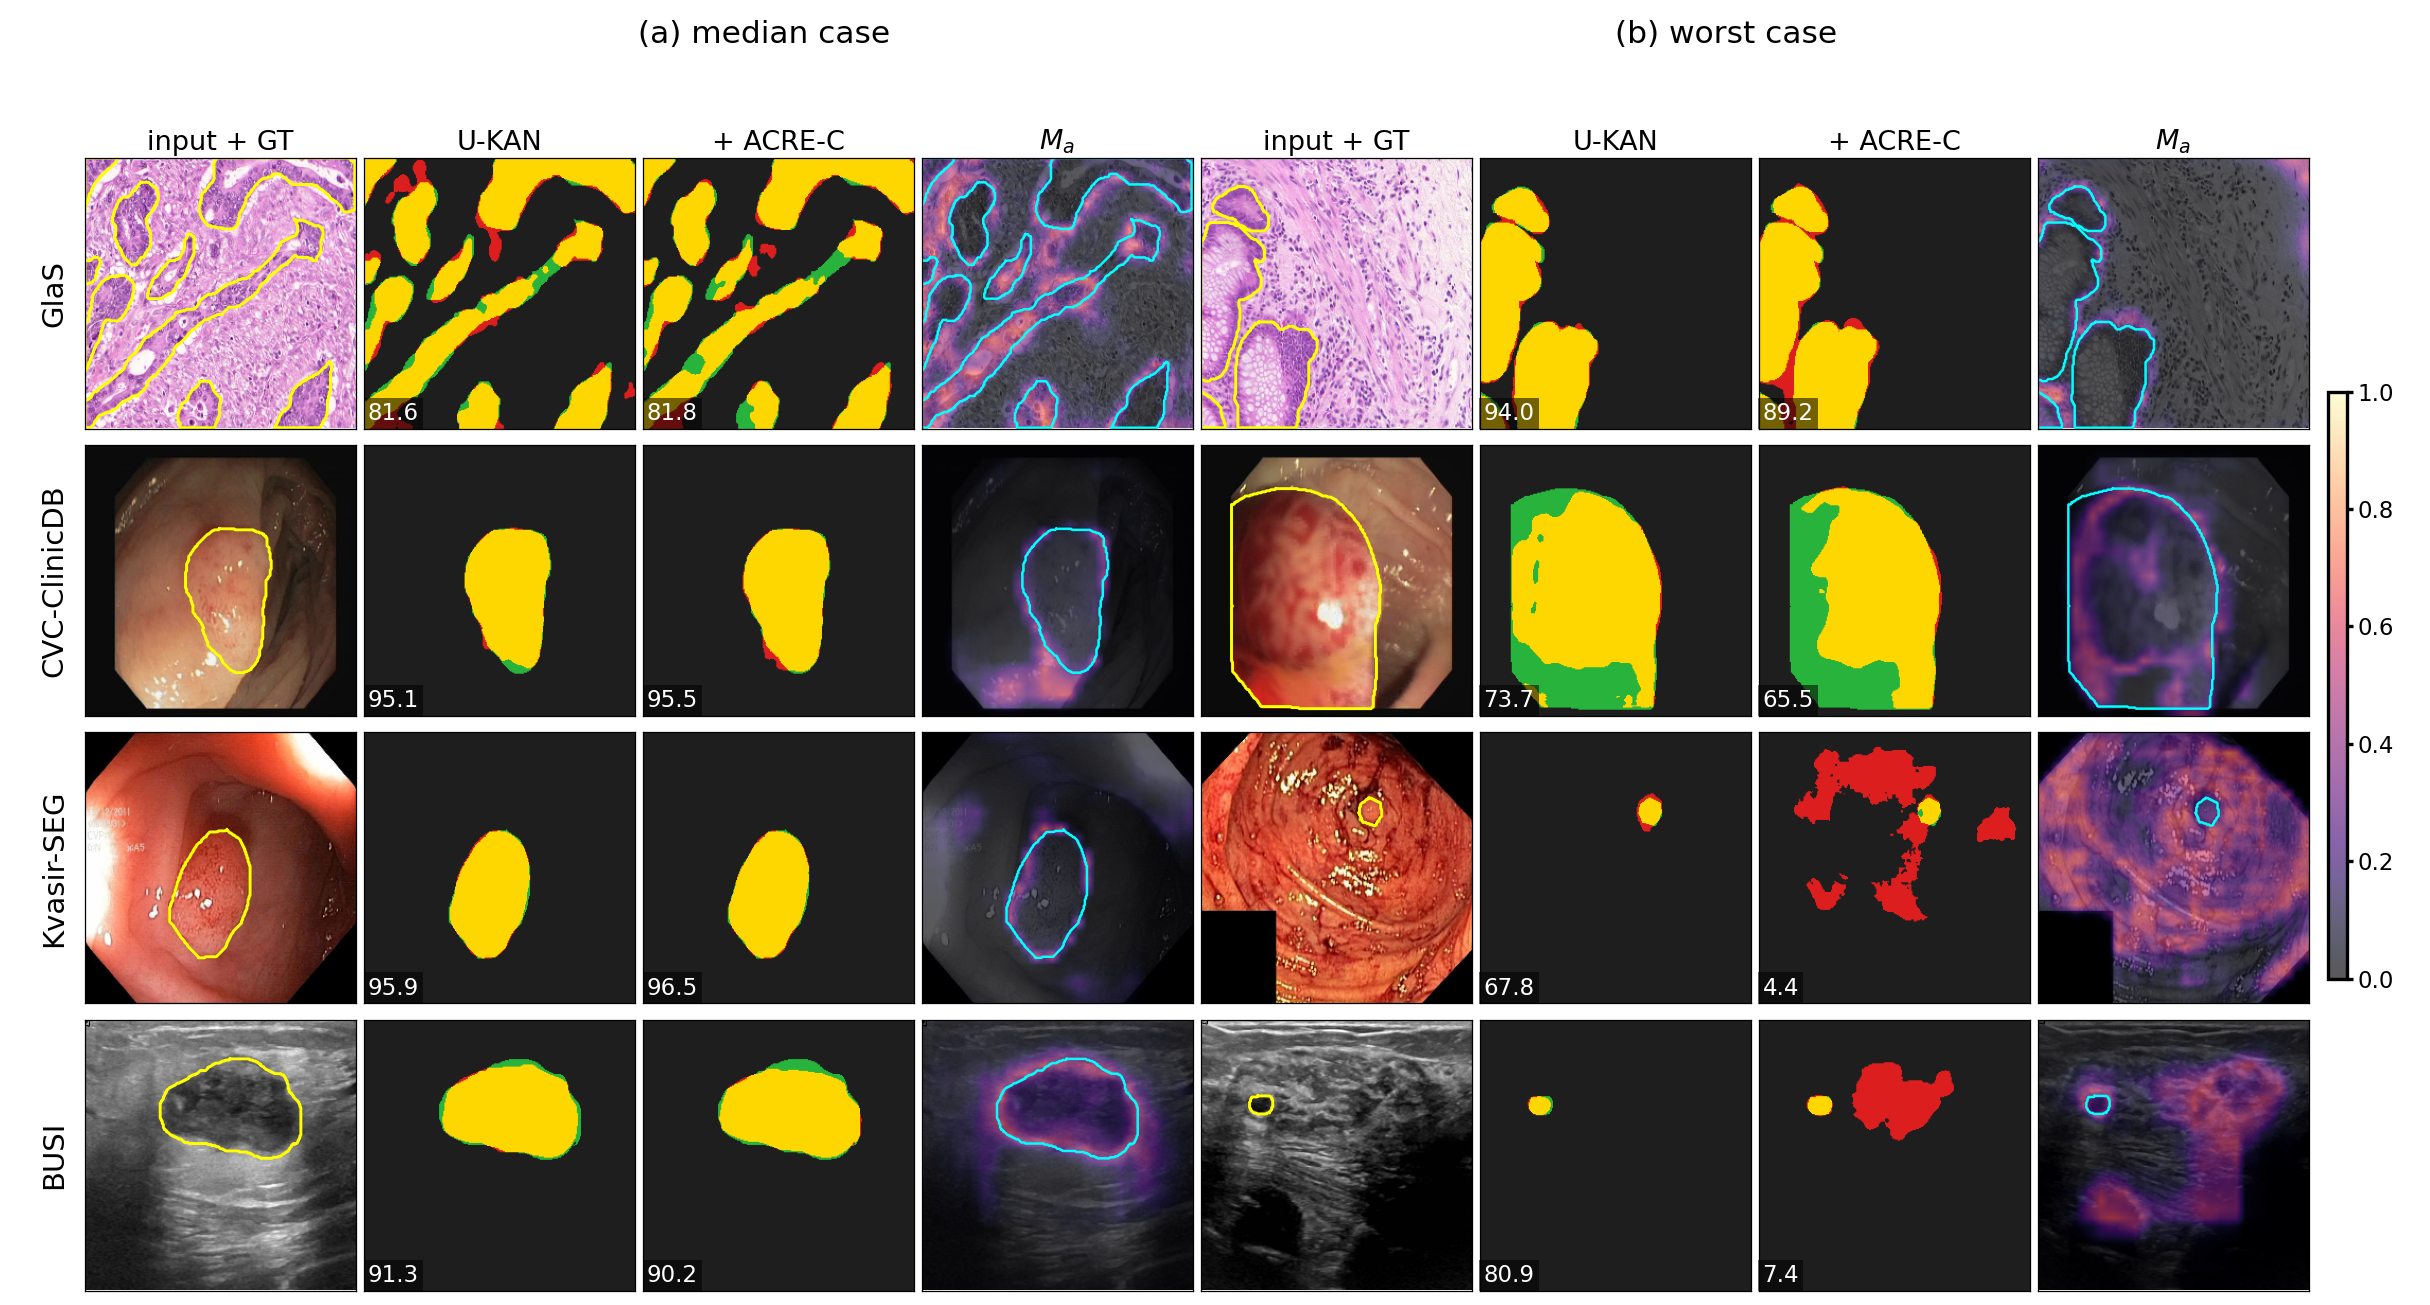
\includegraphics[width=0.75\textwidth]{figures/fig11_qual_grid.png}
\caption{Validation cases of split $2981$, one row per dataset: (a) the image at the median of the per-image IoU difference between the two models, (b) the image with the largest loss against U-KAN. Per block: input with ground-truth contour; error maps of U-KAN and of U-KAN\,+\,ACRE-C (yellow true positive, red false positive, green false negative, per-image IoU inset); the abstention mass $M_a$ ($H/8$ grid, bilinearly resampled) with the ground-truth contour in cyan. Failure cases are shown deliberately.}
\label{fig:qual}
\end{figure*}

Fig.~\ref{fig:qual} shows, for each dataset, the median validation case and the case with the largest loss against the backbone. Two regularities appear in the abstention maps. First, $M_a$ attaches to boundaries: on GlaS it follows the gland contours and the stroma between adjacent glands, on the polyp datasets it forms a rim around the lesion, and on the ultrasound it covers the lesion border and the acoustic shadow beneath it. It is near zero on unambiguous tissue. This is the pattern one expects of a mass that is withheld where the polarity's margin is small, and it was not supervised. Second, the failure cases share one mechanism. On Kvasir-SEG and BUSI the worst cases are a small target inside a large textured field (bleeding mucosa, heterogeneous breast tissue), the polarity abstains over much of that field ($M_a\approx0.3$--$0.5$), and the abstain expert adds false-positive regions there; the backbone, which does not route, does not make them. The worst GlaS and CVC-ClinicDB cases are of a different kind: a contour pushed outward at low $M_a$, and a frame-filling polyp whose left third is missed by both models with $M_a\approx0.3$ over the missed part. The abstention therefore marks where the model is undecided, but the routed expert can also act wrongly there, and the per-image tails of Table~\ref{tab:boundary} on BUSI come from this.

\section{Discussion}
\label{sec:discussion}

\subsection{What the Results Support}

Section~\ref{sec:gates} fixed three screening conditions before any run was started. A pass on gate~(G) means that normalised, abstention-routed fusion keeps what the earlier evidence-routing recipe had gained; a pass on gate~(D) means that the masses read by the routers keep their supervised meaning; gate~(U) is treated below.

One case is complete. On GlaS with data seed $2981$, best validation IoU is $86.36$ against $84.66$ for the re-trained backbone ($+1.70$), and gate~(G) is passed; the mean over the last $50$ epochs rises from $83.48$ to $85.04$ ($+1.56$), so the gain does not rest on checkpoint selection. Over the $33$ validation images (Table~\ref{tab:boundary}), per-image IoU rises from $84.81$ to $86.12$, HD95 falls from $17.67$ to $13.72$ pixels, ASSD from $3.46$ to $3.01$ and BF$_2$ from $73.2$ to $74.1$; $19$ images improve. Across the full protocol the pattern holds on GlaS and Kvasir-SEG: all six seed-level deltas are positive and the boundary metrics move with IoU (HD95 $-3.95$ and $-2.62$ pixels, BF$_2$ $+1.1$ and $+2.7$; Table~\ref{tab:boundary}). On CVC-ClinicDB all three seeds improve in IoU and BF$_2$ while ASSD worsens. On BUSI the sign is not consistent across seeds ($-1.64$, $+0.06$, $+0.22$), matching its level mean; overall, eleven of the twelve seed-level comparisons are positive.

\subsection{What the Abstention Does}

Three observations on the GlaS run bear on the mechanism. First, the polarity did not drift. With $q_{\mathrm{grad}}=0$ the only path from the routers to $p$ is the shared trunk and the encoder feature $t_3$ it reads. Nevertheless the cell-level cross-entropy of $p$ fell from $0.514$ (epochs $50$--$100$) to $0.282$ (last $50$) and the cell IoU rose from $66.1\%$ to $83.2\%$, so gate~(D) is met with margin. The spatial standard deviation of $\rho$ was $0.068$ and the mean abstention mass $\bar M_a=0.165$ (Table~\ref{tab:dynamics}), so neighbouring cells receive different abstention masses, which is the condition under which the routers can act differently across a gland. All twelve full-model runs in Table~\ref{tab:dynamics} behave the same way: $\Delta$BCE between $-0.05$ and $-0.32$, cell IoU rising throughout, and std$(\rho)$ in $0.048$--$0.125$, so the observation is not specific to one run. Second, the expert output-layer norms stayed at or below $2.0$, but their distribution is informative: at $s=3,4$ the abstain expert is larger than the commit expert ($1.99$ and $1.55$ against $0.57$ and $0.29$), while at $s=1,2$ both are approximately $0.7$--$1.0$. At $s=3,4$ the abstain expert, which reads the four contrasts of (\ref{eq:experts}) between the local and image-wide consensuses and the base evidence $u$, has therefore grown more than the commit expert, while at $s=1,2$ the two have grown to similar output-layer norms. Third, $M_a$ concentrates on gland contours and on the stroma between adjacent glands and is close to zero on unambiguous stroma. The worst validation case ($-4.8$ IoU) pushes a gland contour outward where $M_a$ is small, that is, where the controller committed; the failure is a wrong commitment, not an excess of abstention.

What the abstention is not should be stated as plainly. It is not a calibrated uncertainty and not a prediction of error: no target defines it, no loss term takes it as an argument to be matched (the focus loss reads it only under a stop-gradient, Section~\ref{sec:objective}), and there is no coverage decision to trade against accuracy. It is a mass, $m_a=\rho\,\mu$: the fraction $\rho$ of a cell's commitment margin $\mu$ that is withheld from the vote --- $\rho$ receives no direct gradient from any objective, its only coupling to $\mathcal{L}_{\mathrm{ctrl}}$ being the shared trunk; resampled as $M_a$, its only operational content is that abstaining mass does not vote in (\ref{eq:nconv}) and is read by a different expert in (\ref{eq:route}). Part of the contour pattern is structural: the margin $\mu=1-|2q-1|$ vanishes wherever the polarity is confident, so $M_a=\rho\mu$ can be large only near decisions; what is learned is the residual structure of $\rho$ inside that band --- which contours, and which of the two routed experts, gain mass. The pattern is thus a consequence of the construction, not a supervised property.

\subsection{Relation to Prior Selective Fusion}

Gating, attention fusion and generated kernels also condition the skip on a deep state, so a positive delta over the backbone does not by itself separate ACRE-C from them. The separating test is the abstention-policy ablation of Table~\ref{tab:ablation}. Under \emph{none} the router is a two-way consensus driven by a supervised map, the closest analogue within ACRE-C of the two-state routing used by prior designs; under \emph{margin} every cell withholds its full margin, a soft version of the same map. Gate~(U) requires the learned abstention to beat both fixed policies by the $0.2$-point margin fixed in advance in Section~\ref{sec:gates}. Had it beaten neither, the consensus operator alone would carry the result. The outcome on GlaS is intermediate. Against \emph{none} the learned abstention gains $0.68$ points at the best epoch and $0.94$ on the last-$50$ mean, and \emph{none} even falls below the configuration without experts, so a soft third state is what the routers need in order to help. Against \emph{margin} the difference is $+0.23$ at the best epoch and $-0.16$ on the last-$50$ mean: a tie. What the ablation supports is therefore that routing on a withheld margin, rather than on a hard supervised polarity, matters; whether the network learns anything useful in $\rho$ beyond $\rho\equiv1$ is not shown by this single seed. The \emph{margin} policy is a legitimate simplification of ACRE-C, with one parameter fewer, and we report it as such rather than as a defeated alternative. Two further observations qualify the tie without overturning it. Under \emph{margin} the mean abstention mass rises from $0.165$ to $0.226$ (Table~\ref{tab:dynamics}), so the learned $\rho$ withholds less than the full margin at the same overlap. And on the per-image boundary metrics of the best checkpoints the learned policy is ahead: HD95 is $13.72$ pixels against $17.40$ for \emph{margin} and $14.15$ for \emph{none}, ASSD $3.01$ against $3.15$ and $3.05$, while BF$_2$ is within $0.4$ points for all three. The fixed \emph{margin} policy thus matches the learned one in overlap but not in the worst-case contour distance. One seed cannot establish this either, and we leave it as an observation.

\subsection{Limitations}

The evaluation follows the backbone's public $80/20$ protocol, which has no separate test partition and splits at the image level: frames of one colonoscopy sequence in CVC-ClinicDB and images of one patient in BUSI may fall on both sides of the split, so the absolute numbers are protocol-controlled comparisons rather than estimates of patient-level generalisation, and the validation partition is used both for model selection and for reporting (the last-$50$ mean mitigates the selection but does not replace an independent, patient-level-split test cohort). Three data seeds give a paired comparison but little statistical power, and the ladder and side ablations run on GlaS and one seed only, so their transfer to ultrasound and colonoscopy is untested. Only one backbone is instantiated, and the comparison is against the re-trained backbone only: published numbers of other selective-fusion designs are not comparable under this frozen protocol, and running them under it is left as future work. The controller and the four routers together cost $16\%$ more multiply--accumulate operations for $6\%$ more parameters ($0.39$\,M, Table~\ref{tab:params}), and their latency is $17.2$\,ms against $12.0$\,ms for the backbone at batch~1 and $256\times256$ on an idle GPU ($+5.2$\,ms, $+43\%$; Section~\ref{sec:protocol}). Two side ablations point to simplifications that the pre-specified protocol did not allow us to adopt: the fixed \emph{margin} abstention matches the learned one in overlap, and the focus weight built from the label band alone is at least as good as the one that reads the abstention back. A leaner ACRE-C with $\rho\equiv1$ and $\omega=z_{\mathrm{gt}}$ removes one learned map and one stop-gradient path and should be the starting point of any follow-up. The controller is formed on $t_3$ only, so its cells are $8\times8$ input pixels and the abstention at the two shallow scales interpolates a coarser decision; structures thinner than a cell receive no polarity of their own, and forming controllers at finer scales is the direct extension for thin structures. Finally, the formulation is binary: a multi-class extension would need one consensus field per class and a different reading of abstention.

\section{Conclusion}
\label{sec:conclusion}

ACRE-C treats skip fusion as a vote. A controller formed once on the deepest convolutional feature gives every cell a supervised polarity and an abstention with no target. At each decoder scale, commitment-weighted normalised convolution forms a foreground and a background consensus over committed neighbours. The abstention routes the evidence to one of two zero-initialised experts, so the network equals U-KAN at initialisation and departs from the plain sum by a bounded residual. Against the re-trained backbone under the frozen protocol of Section~\ref{sec:protocol}, GlaS (seed $2981$) validation IoU rises by $1.70$ points and HD95 falls from $17.67$ to $13.72$ pixels. Across datasets the three-seed mean IoU deltas are $+0.70$ on GlaS, $+0.62$ on CVC-ClinicDB, $+2.10$ on Kvasir-SEG and $-0.45$ on BUSI, at a cost of $0.39$\,M parameters and $43\%$ more inference latency; the abstention ablation (GlaS, single seed) shows that removing the third state costs $0.68$ points whereas fixing it to the full margin costs nothing measurable, so the soft third state is what the routing needs, and a leaner variant with $\rho\equiv1$ and a label-only focus weight, together with controllers at finer scales for thin structures, is the natural follow-up. These are validation results under a public protocol. Independent test cohorts, a second backbone and multi-seed ablations are required before any claim beyond this evaluation can be made.


\section*{Acknowledgment}
The authors acknowledge the developers of the public U-KAN codebase on which the implementation builds. The experiments use the public BUSI, GlaS, CVC-ClinicDB, and Kvasir-SEG datasets; the implementation (including the initialisation-equivalence unit test), configuration files, complete training logs, and per-run evaluation outputs are publicly available at \url{https://github.com/appleisfalling/science}. Author-specific acknowledgments and funding information will be added before submission.

\bibliographystyle{IEEEtran}
\def\IEEEbibitemsep{0pt plus .5pt}
\bibliography{references,references_v2_additions}

\end{document}
